\documentclass[12pt]{article}
\usepackage{amsmath}
\newcommand{\myvec}[1]{\ensuremath{\begin{pmatrix}#1\end{pmatrix}}}
\newcommand{\mydet}[1]{\ensuremath{\begin{vmatrix}#1\end{vmatrix}}}
\newcommand{\solution}{\noindent \textbf{Solution: }}
\providecommand{\brak}[1]{\ensuremath{\left(#1\right)}}
\providecommand{\norm}[1]{\left\lVert#1\right\rVert}
\let\vec\mathbf
\usepackage{float}
\usepackage{graphicx}

\title{Coordinate Geometry}
\author{Naman Jain(namanjain@sriprakashschools.com)}

\begin{document}
\maketitle
\section*{10$^{th}$ Maths - Chapter 7}
This is Problem-3 from Exercise 7.1
\begin{enumerate}
\item Determine if the points (1, 5), (2, 3) and (-2, -11) are collinear\\ 
\solution \\
\begin{align}
\vec{A}&=\myvec{1\\5}\\
\vec{B}&=\myvec{2\\3}\\
\vec{C}&=\myvec{-2\\-11}\\
\end{align}
Let us assume that these three points are vertices of a triangle. If the given points are collinear, the area of the triangle will be zero.
\\The area of a triangle is given by,
\begin{align}
   &=\frac{1}{2}\norm{\vec{AB}\times\vec{AC}}\\ 
   &=\frac{1}{2}\mydet{1&-3\\-2&-16}\\
   &=\frac{1}{2}\norm{-16-(6)}\\
   &=11\neq 0
\end{align}
Since the area is a non-zero value, the points are not collinear.
\end{enumerate}
\begin{figure}[H]
			\centering
			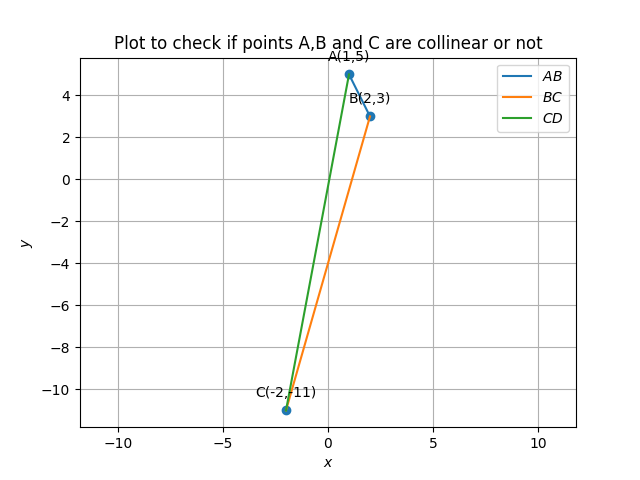
\includegraphics[width=\columnwidth]{figs/Figure_1.png}
			\caption{Points A,B and C aren't collinear}
			\label{fig:20}
		\end{figure}
\end{document}
